% \documentclass[tikz,convert={outfile=\jobname.svg}]{standalone}
\documentclass[tikz,convert=pdf2svg]{standalone}
%\usetikzlibrary{...}% tikz package already loaded by 'tikz' option
\usetikzlibrary{arrows, arrows.meta}
% \tikzset{
%   >=stealth',
% }
\usepackage{amsmath,amssymb}
\usepackage{tikz}
\usepackage{xcolor}

\makeatletter
\def\mathcolor#1#{\@mathcolor{#1}}
\def\@mathcolor#1#2#3{%
  \protect\leavevmode
  \begingroup
    \color#1{#2}#3%
  \endgroup
}
\makeatother

\definecolor{wblue}{HTML}{0072b2}
\definecolor{worange}{HTML}{e69f00}
\definecolor{wbblue}{HTML}{56b4e9}
\definecolor{wgreen}{HTML}{009e73}
\definecolor{wyellow}{HTML}{f0e442}

\begin{document}
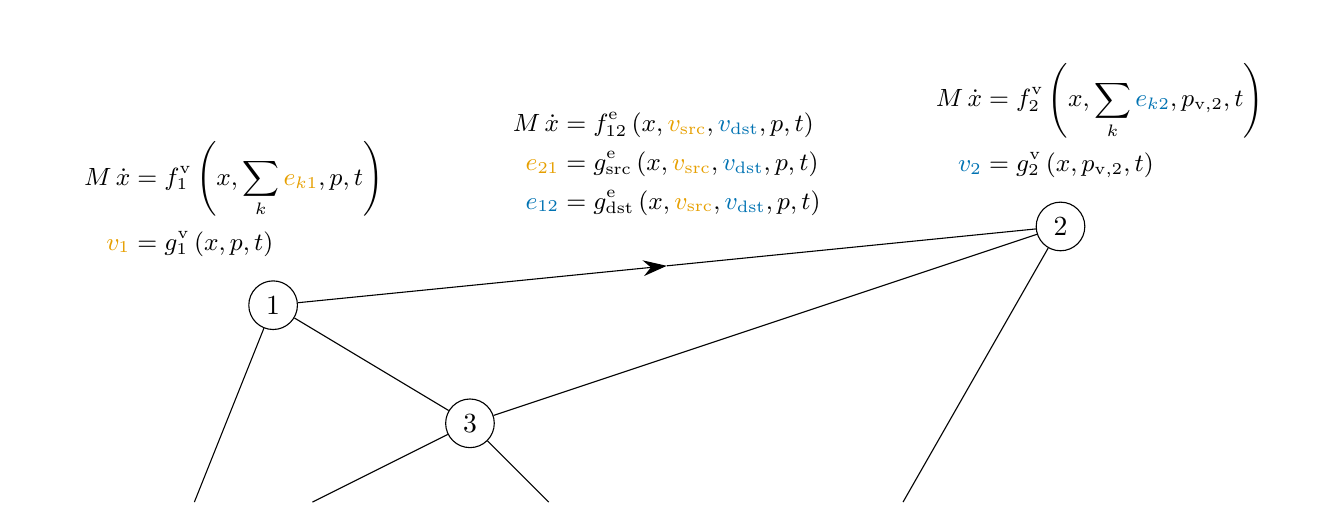
\begin{tikzpicture}
  \node[draw, circle](n1){1};
  \node[draw, circle] at (10cm, 1cm)(n2){2};
  \node[draw, circle] at (2.5cm, -1.5cm)(n3){3};
  \path (n1)--(n2) coordinate[pos=.5](mid12);
  \draw[-{Stealth[length=3mm, width=2mm]}] (n1)--(mid12);
  \draw(mid12)--(n2);
  \draw (n2)--(n3);
  \draw (n3)--(n1);
  \draw[] (n3) --++(-2,-1);
  \draw[] (n3) --++(1,-1);
  \draw[] (n1) --++(-1,-2.5);
  \draw[] (n2) --++(-2,-3.5);

  \node[text width=5cm, xshift=-0.5cm, yshift=1.25cm] at (n1){%
    \small\begin{align*}
    M\,\dot{x} &= f^{\mathrm{v}}_{1}\left(x, \sum_{k} \mathcolor{worange}{e_{k1}}, p, t\right)\\
    \mathcolor{worange}{v_{1}} &= g^{\mathrm{v}}_{1}\left(x, p, t\right)\\
    \end{align*}%
  };
  \node[text width=5cm, xshift=0.5cm, yshift=1.25cm] at (n2)(block){%
    \small\begin{align*}
    M\,\dot{x} &= f^{\mathrm{v}}_{2}\left(x, \sum_{k} \mathcolor{wblue}{e_{k2}}, p_{\mathrm{v},2}, t\right)\\
    \mathcolor{wblue}{v_{2}} &= g^{\mathrm{v}}_{2}\left(x, p_{\mathrm{v},2}, t\right)\\
    \end{align*}%
  };

  \path (n1)--(n2) node[pos=.5,text width=5cm, xshift=0cm, yshift=1.25cm]{%
    \small\begin{align*}
    M\,\dot{x} &= f^{\mathrm{e}}_{12}\left(x, \mathcolor{worange}{v_{\mathrm{src}}}, \mathcolor{wblue}{v_{\mathrm{dst}}}, p, t\right)\\
    \mathcolor{worange}{e_{21}} &= g^{\mathrm{e}}_{\mathrm{src}}\left(x, \mathcolor{worange}{v_{\mathrm{src}}}, \mathcolor{wblue}{v_{\mathrm{dst}}}, p, t\right)\\
    \mathcolor{wblue}{e_{12}} &= g^{\mathrm{e}}_{\mathrm{dst}}\left(x, \mathcolor{worange}{v_{\mathrm{src}}}, \mathcolor{wblue}{v_{\mathrm{dst}}}, p, t\right)\\
    \end{align*}%
  };

\end{tikzpicture}
\end{document}
